
\documentclass{beamer}
\usecolortheme{dove}
\setbeamertemplate{navigation symbols}{}
\usepackage{amsmath,amssymb,amsfonts,amsthm, multicol, subfigure, color}
\usepackage{bm}
\usepackage{graphicx}
\usepackage{tabularx}
\usepackage{booktabs}
\usepackage{hyperref}
\usepackage{pdfpages}
\usepackage{xcolor}
\definecolor{seagreen}{RGB}{46, 139, 87}
\def\independenT#1#2{\mathrel{\rlap{$#1#2$}\mkern2mu{#1#2}}}
\newcommand\indep{\protect\mathpalette{\protect\independenT}{\perp}}
\def\log{\text{log}}
\newcommand\logit{\text{logit}}
\newcommand\iid{\stackrel{\text{iid}}{\sim}}
\newcommand\E{\text{E}}
\newcommand\V{\text{V}}
\renewcommand\P{\text{P}}
\newcommand{\Cov}{\text{Cov}}
\newcommand{\Cor}{\text{Cor}}
\newcommand\doop{\texttt{do}}
\usepackage{stackrel}
\usepackage{tikz}
\usetikzlibrary{arrows,shapes.arrows,positioning,shapes,patterns,calc}
\newcommand\slideref[1]{\vskip .1cm \tiny \textcolor{gray}{{#1}}}
\newcommand\red[1]{\color{red}#1}
\newcommand\blue[1]{\color{blue}#1}
\newcommand\gray[1]{\color{gray}#1}
\newcommand\seagreen[1]{\color{seagreen}#1}
\newcommand\purple[1]{\color{purple}#1}
\newcommand\orange[1]{\color{orange}#1}
\newcommand\black[1]{\color{black}#1}
\newcommand\white[1]{\color{white}#1}
\newcommand\teal[1]{\color{teal}#1}
\newcommand\magenta[1]{\color{magenta}#1}
\newcommand\Fuchsia[1]{\color{Fuchsia}#1}
\newcommand\BlueGreen[1]{\color{BlueGreen}#1}
\newcommand\bblue[1]{\textcolor{blue}{\textbf{#1}}}
\newcommand\bred[1]{\textcolor{red}{\textbf{#1}}}
\newcommand\bgray[1]{\textcolor{gray}{\textbf{#1}}}
\newcommand\bgreen[1]{\textcolor{seagreen}{\textbf{#1}}}
\newcommand\bref[2]{\href{#1}{\color{blue}{#2}}}
\colorlet{lightgray}{gray!40}
\pgfdeclarelayer{bg}    % declare background layer for tikz
\pgfsetlayers{bg,main} % order layers for tikz
\newcommand\mycite[1]{\begin{scriptsize}\textcolor{darkgray}{(#1)}\end{scriptsize}}
\newcommand{\tcframe}{\frame{
%\small{
\only<1|handout:0>{\tableofcontents}
\only<2|handout:1>{\tableofcontents[currentsubsection]}}
%}
}

\usepackage[round]{natbib}
\bibliographystyle{humannat-mod}
\setbeamertemplate{enumerate items}[default]
\usepackage{mathtools}
\usepackage{ulem}

% Need to add examples

\newcommand{\goalsframe}{\begin{frame}{Learning goals for today}
At the end of class, you will be able to:
\begin{enumerate}
\item Recognize differences between DAGs and linear path models
\item Determine the covariance between standardized variables using a linear path model
\item Quantify the biases of coefficient estimators using path models
\item Be equipped to read Elwert \& Pfeffer (2022)
\end{enumerate} \vskip .2in
\end{frame}}

\title{24. From DAGs to linear path models}
\author{Ian Lundberg\\Cornell Info 6751: Causal Inference in Observational Settings\\Fall 2022}
\date{15 Nov 2022}

\begin{document}

\maketitle

\goalsframe

\begin{frame}{We have been working with DAGs}

\begin{center}
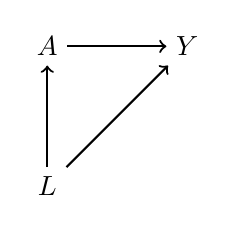
\begin{tikzpicture}[x = .7in, y = .7in]
\node (l) at (0,-1) {$L$};
\node (a) at (0,0) {$A$};
\node (y) at (1,0) {$Y$};
\draw[->, thick] (l) -- (a);
\draw[->, thick] (a) -- (y);
\draw[->, thick] (l) -- (y);
\end{tikzpicture}
\end{center}

\begin{itemize}
\item Each node is a variable
\item Each edge is a direct causal effect
\item The DAG is nonparametric
\begin{itemize}
\item Effect of $A$ may be nonlinear
\item Effect of $A$ may be heterogeneous across $L$
\end{itemize}
\end{itemize} \vskip .1in
$$\E(Y\mid A, L) = f(A,L) \qquad \leftarrow \text{arbitrarily complex }f()$$

\end{frame}

\begin{frame}{Today we will use linear path models} \pause

\begin{center}
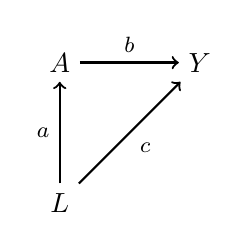
\begin{tikzpicture}[x = .7in, y = .7in]
\node (l) at (0,-1) {$L$};
\node (a) at (0,0) {$A$};
\node (y) at (1,0) {$Y$};
\draw[->, thick] (l) -- node[midway, left, font = \footnotesize] {$a$} (a);
\draw[->, thick] (a) -- node[midway, above, font = \footnotesize] {$b$} (y);
\draw[->, thick] (l) -- node[midway, below right, font = \footnotesize] {$c$} (y);
\end{tikzpicture}
\end{center} \pause

Adds a \bgray{parametric assumption:}\\
Each output is a linear, additive function of its inputs \pause
$$\E(Y\mid A, L) = \alpha + bA + cL$$ \pause \vspace{-.2in}
\begin{itemize}
\item Homogeneous causal effects \pause
\item Linear causal effects \pause
\end{itemize}
\vskip .1in
We will also assume all variables are \bgray{standardized}\\to mean 0 and variance 1

\end{frame}

\begin{frame}

\centering
\includegraphics[height = \textheight]{figures/wright1921_p1}

\end{frame}

\begin{frame}{Wright's (1921) path rule:\\Connecting causal paths to statistical associations}

\begin{center}
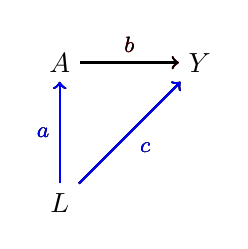
\begin{tikzpicture}[x = .7in, y = .7in]
\node (l) at (0,-1) {$L$};
\node (a) at (0,0) {$A$};
\node (y) at (1,0) {$Y$};
\onslide<1,6->{
\draw[->, thick] (l) -- node[midway, left, font = \footnotesize] {$a$} (a);
\draw[->, thick] (a) -- node[midway, above, font = \footnotesize] {$b$} (y);
\draw[->, thick] (l) -- node[midway, below right, font = \footnotesize] {$c$} (y);
}
\onslide<2-3>{
\draw[->, thick] (l) -- node[midway, left, font = \footnotesize] {$a$} (a);
\draw[->, thick, red] (a) -- node[midway, above, font = \footnotesize] {$b$} (y);
\draw[->, thick] (l) -- node[midway, below right, font = \footnotesize] {$c$} (y);
}
\onslide<4-5>{
\draw[->, thick, blue] (l) -- node[midway, left, font = \footnotesize] {$a$} (a);
\draw[->, thick] (a) -- node[midway, above, font = \footnotesize] {$b$} (y);
\draw[->, thick, blue] (l) -- node[midway, below right, font = \footnotesize] {$c$} (y);
}
\end{tikzpicture}
\end{center} 

$$\Cov(A,\tilde{Y}) = \onslide<3->{\red{b}}\onslide<5->{\black{ + }\blue{ac}}$$

\onslide<6->{
\bgray{Wright's rule:}\\When all variables are standardized to variance 1,\\the covariance between two variables\\is the sum over unblocked paths\\of the product of coefficients on that path
}

\end{frame}

\begin{frame}{Quick practice}
Wright's rule:\\The covariance is the sum over unblocked paths\\of the product of coefficients on each path
\begin{center}
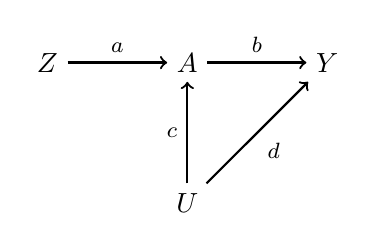
\begin{tikzpicture}[x = .7in, y = .7in]
\node (z) at (-1,0) {$Z$};
\node (u) at (0,-1) {$U$};
\node (a) at (0,0) {$A$};
\node (y) at (1,0) {$Y$};
\draw[->, thick] (z) -- node[midway, above, font = \footnotesize] {$a$} (a);
\draw[->, thick] (u) -- node[midway, left, font = \footnotesize] {$c$} (a);
\draw[->, thick] (a) -- node[midway, above, font = \footnotesize] {$b$} (y);
\draw[->, thick] (u) -- node[midway, below right, font = \footnotesize] {$d$} (y);
\end{tikzpicture}
\end{center}
$$\begin{aligned}
\Cov(Z,A) &= \only<1>{?}\onslide<2->{
a
}
\\
\Cov(Z,Y) &= \only<1-2>{?}\onslide<3->{
ab
}\\
\end{aligned}$$
\onslide<4->{ \vskip .3in
\bgray{Note.} $\frac{\Cov(Z,Y)}{\Cov(Z,A)} \onslide<5->{ = \frac{ab}{a}} \onslide<6->{ = b$}\onslide<7->{ \hfill Stay tuned...future class!}
}
\end{frame}

\begin{frame}[t]{When is Wright's rule helpful? Reasoning about biases}

\begin{center}
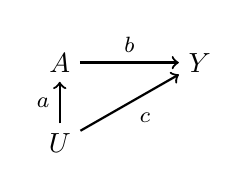
\begin{tikzpicture}[x = .7in, y = .4in]
\node (l) at (0,-1) {$U$};
\node (a) at (0,0) {$A$};
\node (y) at (1,0) {$Y$};
%\node (ytilde) at (1,-1) {$\tilde{Y}$};
\draw[->, thick] (l) -- node[midway, left, font = \footnotesize] {$a$} (a);
\draw[->, thick] (a) -- node[midway, above, font = \footnotesize] {$b$} (y);
\draw[->, thick] (l) -- node[midway, below right, font = \footnotesize] {$c$} (y);
%\draw[->, thick] (y) -- node[midway, right, font = \footnotesize] {$\eta_{Y\tilde{Y}}$} (ytilde);
\end{tikzpicture}
\end{center} 

Suppose we don't observe $U$. \pause We regress $Y$ on $A$.
$$\E(Y\mid A) = \alpha + \beta A$$ \pause
What do we get? \pause
$$\begin{aligned}
\beta &= \frac{\Cov(A,Y)}{\V(Y)} &\text{from regression} \\ \pause
&= \Cov(A,Y) &\text{since standardized} \\ \pause
&= \underbrace{b}_\text{Estimand} + \underbrace{ac}_\text{Bias} &\text{Wright's rule}
\end{aligned}$$

\end{frame}

\begin{frame}{When is Wright's rule helpful? Reasoning about biases}

\bgray{Discuss.}\\
Think about that bias in a substantive example.

\end{frame}

\begin{frame}{Conditional estimators meet Wright's rule}

\begin{tikzpicture}[x = \textwidth, y = .8\textheight]
\node at (0,0) {};
\node at (1,1) {};
\node[anchor = north west] at (0,.8) {$\E(Y\mid A,L) = \alpha + \beta A + \gamma L$};
\node[anchor = north] at (.15, .7) {\begin{tikzpicture}[x = .7in, y = .4in, every node/.style = {anchor = center}]
\node (l) at (0,-1) {$L$};
\node (a) at (0,0) {$A$};
\node (y) at (1,0) {$Y$};
%\node (ltilde) at (0,-2) {$\tilde{L}$};
\draw[->, thick] (l) -- node[midway, left, font = \footnotesize] {$a$} (a);
\draw[->, thick] (a) -- node[midway, above, font = \footnotesize] {$b$} (y);
\draw[->, thick] (l) -- node[midway, above left, font = \footnotesize] {$c$} (y);
%\draw[->, thick] (l) -- node[midway, right, font = \footnotesize] {$d$} (ltilde);
\end{tikzpicture}}; \pause
\node[anchor = north west, font = \footnotesize, align = left] at (.5, .8) {$\begin{aligned}
\beta &= \frac{\Cov(A,Y) - \Cov(L,Y)\Cov(L,A)}{1 - \left[\Cov(L,A)\right]^2} \\ \pause
&= \frac{\big(b + ac\big) - \big((c + ab)a\big)}{1 - a^2} \\ \pause
&= \frac{b + ac - ac - a^2b}{1 - a^2} \\ \pause
&= \frac{b(1 - a^2)}{1 - a^2}\\ \pause
&= b
\end{aligned}$};
%\node[anchor = north west, font = \footnotesize, align = left] at (0,.3) {\bgray{Result.}\\If you don't measure $L$,\\then controlling for $\tilde{L}$\\is strictly better than\\controlling for nothing};
\end{tikzpicture}

\end{frame}

% TRANSITION SLIDE TO TAKE THINGS AWAY BEFORE ADDING
\begin{frame}{Conditional estimators meet Wright's rule}

\begin{tikzpicture}[x = \textwidth, y = .8\textheight]
\node at (0,0) {};
\node at (1,1) {};
\node[anchor = north west] at (0,.8) {$\E(Y\mid A,L) = \alpha + \beta A + \gamma L$};
\node[anchor = north] at (.15, .7) {\begin{tikzpicture}[x = .7in, y = .4in, every node/.style = {anchor = center}]
\node (l) at (0,-1) {$L$};
\node (a) at (0,0) {$A$};
\node (y) at (1,0) {$Y$};
\draw[->, thick] (l) -- node[midway, left, font = \footnotesize] {$a$} (a);
\draw[->, thick] (a) -- node[midway, above, font = \footnotesize] {$b$} (y);
\draw[->, thick] (l) -- node[midway, above left, font = \footnotesize] {$c$} (y);
\end{tikzpicture}};
\end{tikzpicture}
\end{frame}

\begin{frame}{Conditional estimators meet Wright's rule}

\begin{tikzpicture}[x = \textwidth, y = .8\textheight]
\node at (0,0) {};
\node at (1,1) {};
\node[anchor = north west] at (0,.8) {$\E(Y\mid A,\tilde{L}) = \alpha + \beta A + \gamma \tilde{L}$};
\node[anchor = north] at (.15, .7) {\begin{tikzpicture}[x = .7in, y = .4in, every node/.style = {anchor = center}]
\node (l) at (0,-1) {$L$};
\node (a) at (0,0) {$A$};
\node (y) at (1,0) {$Y$};
\draw[->, thick] (l) -- node[midway, left, font = \footnotesize] {$a$} (a);
\draw[->, thick] (a) -- node[midway, above, font = \footnotesize] {$b$} (y);
\draw[->, thick] (l) -- node[midway, above left, font = \footnotesize] {$c$} (y);
\node (ltilde) at (1,-1) {$\tilde{L}$};
\draw[->, thick] (l) -- node[midway, below, font = \footnotesize] {$d$} (ltilde);
\end{tikzpicture}};
\pause
\node[anchor = north west, font = \footnotesize, align = left] at (.5, .8) {$\begin{aligned}
\beta &= \frac{\Cov(A,Y) - \Cov(\tilde{L},Y)\Cov(\tilde{L},A)}{1 - \left[\Cov(\tilde{L},A)\right]^2} \\ \pause
&= \frac{\big(b + ac\big) - \big((cd + abd)ad\big)}{1 - a^2d^2} \\ \pause
&= \frac{b + ac - acd^2 - a^2bd^2}{1 - a^2d^2} \\ \pause
&= \frac{b(1 - a^2d^2) + ac(1 - d^2)}{1 - a^2d^2} \\ \pause
&= b + \underbrace{ac}_{\substack{\text{Bias}\\\text{without}\\\text{control}}}\underbrace{\frac{1 - d^2}{1 - a^2d^2}}_{\substack{\text{Bias}\\\text{Multiplier}\\<1}} \\
\end{aligned}$};
\node<7->[anchor = north west, font = \footnotesize, align = left] at (0,.3) {\bgray{Result.}\\If you don't measure $L$,\\then controlling for $\tilde{L}$\\is strictly better than\\controlling for nothing};
\end{tikzpicture}


\end{frame}

\begin{frame}{Elwert \& Pfeffer 2022}

\begin{tikzpicture}
\node[anchor = east] at (0,0) {\includegraphics[height = .8\textheight]{figures/ep_p1}};
\node<2>[anchor = west] at (0,0) {\includegraphics[width = .4\textwidth]{figures/ep_fig1}};
\end{tikzpicture}

\end{frame}

\begin{frame}{Elwert \& Pfeffer 2022}
\begin{center}
\includegraphics[width = .4\textwidth]{figures/ep_fig1}
\only<2>{\includegraphics[width = .5\textwidth]{figures/ep_fig3}}
\end{center}
$$\E(Y\mid T, F) = \alpha + \beta T + \gamma F$$
Two estimators:
\begin{enumerate}
\item Control estimator: $\beta$
\item Difference estimator: $\beta - \gamma$
\end{enumerate}
\end{frame}

\begin{frame}{Elwert \& Pfeffer 2022}
\centering
\includegraphics[width = .4\textwidth]{figures/ep_fig1}
\includegraphics[width = .5\textwidth]{figures/ep_fig3}
\end{frame}

\begin{frame}{Reading before Thursday}
Elwert, F., \& Pfeffer, F. T. (2022). \bref{https://doi.org/10.1177/0049124119875958}{The future strikes back: using future treatments to detect and reduce hidden bias.} Sociological Methods \& Research, 51(3), 1014-1051.
\end{frame}

\begin{frame}{More practice with path diagrams}
\begin{tikzpicture}[x = \textwidth, y = .8\textheight]
\node at (0,0) {};
\node at (1,1) {};
\node[anchor = north] at (.15, .8) {\begin{tikzpicture}[x = .7in, y = .4in, every node/.style = {anchor = center}]
\node (z) at (-1,0) {$Z$};
\node (u) at (0,-1) {$U$};
\node (a) at (0,0) {$A$};
\node (y) at (1,0) {$Y$};
\draw[->, thick] (z) -- node[midway, above, font = \footnotesize] {$a$} (a);
\draw[->, thick] (u) -- node[midway, left, font = \footnotesize] {$c$} (a);
\draw[->, thick] (a) -- node[midway, above, font = \footnotesize] {$b$} (y);
\draw[->, thick] (u) -- node[midway, below right, font = \footnotesize] {$d$} (y);
\end{tikzpicture}};
\onslide<2->{
\node[anchor = north west, align = left] (n1) at (0,.4) {What is $\Cov(A,Y)$?\\\only<3->{$b + cd$}};
\node[anchor = north west, align = left] (n2) at (n1.south west) {What is $\Cov(Z,A)$?\\\only<4->{$a$}};
\node[anchor = north west, align = left] at (n2.south west) {What is $\Cov(Z,Y)$?\\\only<5->{$ab$}};
}
\node[anchor = north west, font = \footnotesize] at (.5,.9) {$\begin{aligned}
\beta_\text{Unadjusted} &= \Cov(A,Y) \\
\only<6->{&= \underbrace{b}_\text{Effect} + \underbrace{cd}_\text{Bias}}
\end{aligned}$};
\node[anchor = north west, font = \footnotesize] at (.5,.6) {$\begin{aligned}
&\beta_\text{Adjusted}\\
\only<7->{&= \frac{\Cov(A,Y) - \Cov(Z,Y)\Cov(Z,A)}{1 - \left[\Cov(Z,A)\right]^2}} \\
\only<8->{&= \frac{(b + cd) - (ab)(a)}{1 - a^2}} \\
\only<9->{&= \frac{b(1 - a^2) + cd}{1 - a^2}} \\
\only<10->{&= \underbrace{b}\only<11->{_\text{Effect}} + \underbrace{cd}\only<12->{_\text{Bias}}\underbrace{\frac{1}{1 - a^2}}\only<13->{_{\substack{\text{Bias}\\\text{Amplifier}\\\geq1}}}}
\end{aligned}$};
\end{tikzpicture}

\end{frame}


\begin{frame}{What we have learned}
\begin{tikzpicture}[x = \textwidth, y = .8\textheight]
\node at (0,0) {};
\node at (1,1) {};
\node[anchor = north] (bias) at (.9,1) {Bias};
\draw[thick] (bias.south west) -- (bias.south east);
% Quantify
\node[anchor = north west, align = left] at (0,.9) {We can quantify the bias\\from unmeasured variables};
\node[anchor = north] at (.9,.9) {$ac$};
\node[anchor = north] at (.6, .95) {\begin{tikzpicture}[x = .7in, y = .4in, every node/.style = {anchor = center}]
\node (l) at (0,-1) {$U$};
\node (a) at (0,0) {$A$};
\node (y) at (1,0) {$Y$};
\draw[->, thick] (l) -- node[midway, left, font = \footnotesize] {$a$} (a);
\draw[->, thick] (a) -- node[midway, above, font = \footnotesize] {$b$} (y);
\draw[->, thick] (l) -- node[midway, below right, font = \footnotesize] {$c$} (y);
\end{tikzpicture}};
% Reduce
\node[anchor = north west, align = left] at (0,.6) {We can reduce the bias\\by adjusting for a proxy};
\node[anchor = north] at (.9,.6) {$ac\frac{1 - d^2}{1-a^2d^2}$};
\node[anchor = north] at (.6, .65) {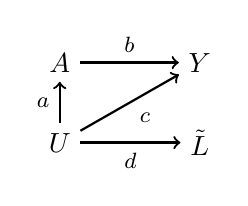
\begin{tikzpicture}[x = .7in, y = .4in, every node/.style = {anchor = center}]
\node (l) at (0,-1) {$U$};
\node (a) at (0,0) {$A$};
\node (y) at (1,0) {$Y$};
\draw[->, thick] (l) -- node[midway, left, font = \footnotesize] {$a$} (a);
\draw[->, thick] (a) -- node[midway, above, font = \footnotesize] {$b$} (y);
\draw[->, thick] (l) -- node[midway, below right, font = \footnotesize] {$c$} (y);
\node (ltilde) at (1,-1) {$\tilde{L}$};
\draw[->, thick] (l) -- node[midway, below, font = \footnotesize] {$d$} (ltilde);
\end{tikzpicture}};
% Discover
\node[anchor = north west, align = left] at (0,.3) {We can do many things!\\Example:\\Bad controls magnify bias};
\node[anchor = north] at (.9,.3) {$cd\frac{1}{1 - a^2}$};
\node[anchor = north] at (.6, .35) {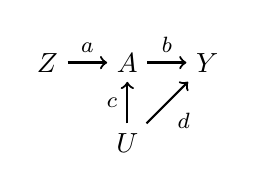
\begin{tikzpicture}[x = .4in, y = .4in, every node/.style = {anchor = center}]
\node (z) at (-1,0) {$Z$};
\node (u) at (0,-1) {$U$};
\node (a) at (0,0) {$A$};
\node (y) at (1,0) {$Y$};
\draw[->, thick] (z) -- node[midway, above, font = \footnotesize] {$a$} (a);
\draw[->, thick] (u) -- node[midway, left, font = \footnotesize] {$c$} (a);
\draw[->, thick] (a) -- node[midway, above, font = \footnotesize] {$b$} (y);
\draw[->, thick] (u) -- node[midway, below right, font = \footnotesize] {$d$} (y);
\end{tikzpicture}};
\end{tikzpicture}
\end{frame}

\begin{frame}
Cost of all of these things: Linear path model
\begin{itemize}
\item Homogeneous causal effects
\item Linear causal effects
\end{itemize}
$$\E(Y\mid A, L) = \alpha + \beta_1 A + \beta_2 L$$
\end{frame}

\goalsframe

\begin{frame}{Let me know what you are thinking}

\begin{huge} \bref{https://tinyurl.com/CausalQuestions}{tinyurl.com/CausalQuestions} \end{huge}
\vskip .7in

Office hours TTh 11am-12pm and at \bref{https://calendly.com/ianlundberg/office-hours}{calendly.com/ianlundberg/office-hours}\\Come say hi!

\end{frame}

\end{document}


